\section{Introduction and general overview}
\subsection{What is Deep Learning?}
\begin{quotation}
    \textit{Deep learning is constructing networks of parameterized functional modules \& training them from examples using gradient-based optimization.}\hfill--- Yann Le Cun
\end{quotation}

\subsubsection{Neural networks}
The notion of neural networks changed over the last height decades. Early neural networks aimed at imitating real neurons from the brain; today, neural networks involve highly complex architectures with multiple submodules.

Nevertheless, the fundamental idea of deep learning remains the same: a neural network represents a parameterized function, no matter how complex its architecture is. The parameters of the function are learned from data using optimization algorithms, such as gradient descent. The beauty of deep learning holds in the fact that the function can be arbitrarily complex, as long as it is differentiable: if we can evaluate its gradient on data samples, we can optimize it.

\subsubsection{Timeline of Deep Learning}
\begin{figure}[H]
    \centering
    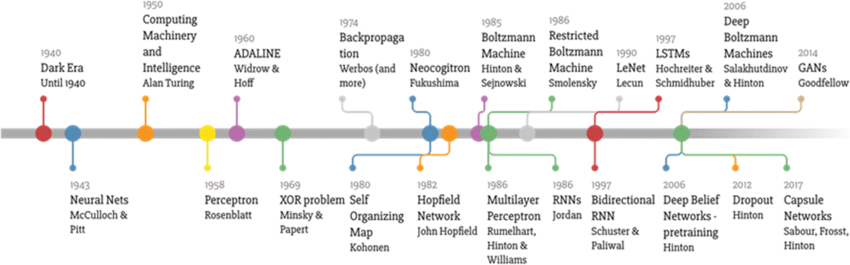
\includegraphics[width=0.8\textwidth]{introduction/timeline.png}
    \caption{Timeline of Deep Learning.}
\end{figure}

\subsubsection{Recent applications and breakthroughs}
Deep learning has been applied to a wide range of fields, including computer vision, natural language processing, speech recognition, and reinforcement learning. Some of the most notable breakthroughs include:
\begin{itemize}
    \item \textbf{Voice, audio, and music generation} with models such as MusicGen, MusicLM, MusicLDM, Jukebox, and HeyGen.
    \item \textbf{Voice to text} with Whisper
    \item \textbf{Image generation} with products such as DALL-E, MidJourney, Stable Diffusion
    \item \textbf{Text generation} with chatbots such as ChatGPT, GPT4, LLaMa, Claude, or Mistral
    \item \textbf{Video generation} with Make-a-video, HeyGEn
    \item \textbf{Code generation} through Codex, Code LLaMa, or AutoGPT
    \item \textbf{Strategy games} with AlphaZero, LeelaChess, Cicero
    \item \textbf{Autonomous driving}
    \item \textbf{Protein folding} with AlphaFold
    \item \ldots  
\end{itemize}

Most recent breakthroughs, particularly noted by the public, include rapid improvements in natural language processing, such as the GPT-3 model, which can generate human-like text, or in image generation, such as the DALL-E model, which can generate images from textual descriptions.

\subsubsection{Building blocks of deep learning}
A deep learning pipeline typically involves three major steps:
\begin{enumerate}
    \item \textbf{Data loading and pre-processing}: data is loaded from a source and pre-processed to be fed into the model. This step may involve data augmentation, normalization, and splitting into training and validation sets or mini-batches. More complex transformations involve encoding layers, tokenization, or embeddings.
    \item \textbf{Model creation}: a deep neural network is created usually from a set of building blocks. Different types of layers are stacked together to form the model. The model may involve convolutional layers, recurrent layers, attention layers, batch normalization, \dots
    \item \textbf{Training}: an algorithm is chosen to optimize the parameters of the model. The most common algorithm is gradient descent, but variations such as stochastic gradient descent, Adam, or RMSprop are also used. The training process involves feeding the model with data samples, computing the loss, and updating the parameters of the model using the gradients of the loss with respect to the parameters. Other techniques such as weight initialization, scheduling, or hyperparameter optimization are also used to improve the training process.
\end{enumerate}

\subsubsection{Why deep learning now?}
Research in deep learning has been ongoing for approximately five decades, but it has only recently gained significant traction. The main reason for this has been the availability of computational power: CPUs, GPUs and storage devices have been developped for other purposes, and especially computer gaming, but they have been repurposed for deep learning. 

The availability of large datasets has also been a key factor in the success of deep learning, thanks to the internet and the massive digitization of data. For instance, the ImageNet dataset, which contains millions of labeled images, has been a key factor in the success of deep learning in computer vision. The constitution of such datasets would have been impossible without the internet.

Finally, deep learning has been pushed forward by large corporations through ressources and efforts. Tools, libraries, and the culture of collaborative and reproducible research have been developed by companies such as Google, Facebook, Microsoft, and OpenAI.

\subsection{Machine Learning pipeline}
\subsubsection{Typical Machine Learning setup}
Let $\X, \Y$ be an input and output space, and $\D$ a distribution over $\X\times\Y$. Then, we denote our test (input, output) pair as
\begin{equation*}
    (X, Y) \sim \D
\end{equation*}

Our intuitive goal is to build a model $g:\X\to\Y$ such that given the outcome of $X$, the pair $(X, g(X))$ is as close as possible to $(X, Y)$. To do so, we choose a class of parameterized functions $g_\theta$, and choose the best possible parameter $\theta$.

Formally, the objective of \emph{risk minimization} is to find a minimizer $\theta^*\in\R^p$ of the following optimization problem:
\begin{equation*}
    \min_{\theta\in\R^p} \E\left[\ell(g_\theta(X), Y)\right]
\end{equation*}
where $\ell:\Y^2\to\R_+$ is a loss function, and $g_\theta:\X\to\Y$ is a model parameterized by $\theta\in\R^p$.

Note that the target loss (for instance, the accuracy) may be hard to train, and can thus be different from the one used as objective during training. For instance, the 0-1 loss is not differentiable, and thus cannot be used as a loss function for gradient-based optimization.

The accuracy is given by:
\begin{equation*}
    \ell(y, y') = \ind_{y\neq y'}
\end{equation*}
For classification tasks, where $\Y=\R^C$ for $C$ the number of classes, the cross-entropy loss is often used:
\begin{equation*}
    \ell(y, y') = -\sum_{c=1}^C y_i' \log\left(\exp(y_i) / \sum_{c'=1}^C \exp(y_{c'})\right)
\end{equation*}
Even though we could have used the accuracy as a loss function:
\begin{equation*}
    \ell(y, y') = \ind_{\argmax(y) \neq \argmax(y')}
\end{equation*}
this function is not differentiable, and thus cannot be used for gradient-based optimization. Intuitively, the accuracy is too strict, since it does not take into account the confidence of the model in its prediction.

Similarly, for regression tasks where $\Y=\R^d$, the mean squared error is often used:
\begin{equation*}
    \ell(y, y') = \norm{y-y'}^2_2 = \sum_i (y_i-y'_i)^2
\end{equation*}

\subsubsection{Training objective}
In practice, we cannot compute the expectation of the loss over the distribution $\D$, since it is unknown. Instead, we use the empirical risk minimization principle, which states that the empirical risk is a good approximation of the true risk.

Let $(x_i, y_i)_{i\in\iset{1}{n}}$ be a collection of $n$ observations independently drawn from $\D$. Then, the objective of \emph{empirical risk minimization} is to find a minimizer $\htheta^*\in\R^p$ of the following optimization problem:
\begin{equation*}
    \min_{\theta\in\R^p} \frac{1}{n} \sum_{i=1}^n \ell(g_\theta(x_i), y_i)
\end{equation*}

We can minimize this loss by iteration the following operation:
\begin{equation*}
    \theta_{t+1} = \theta_t - \eta \nabla_\theta \hat{\L}_n(\theta_t)
\end{equation*}
where $\eta>0$ is a fixed step-size and $\hat{\L}_n(\theta)=\frac{1}{n}\sum_{i=1}^n\ell(g_{\theta}(x_i), y_i)$ is the empirical loss.

We will see in more details in the next sections how this optimization problem can be solved using various gradient-based optimization algorithms.

\subsection{Multi-Layer Perceptron}
\subsubsection{Definition}
The multi-layer perceptron (MLP) is the first and simplest type of neural network. It is composed of an alternating sequence of linear layers and non-linear activation functions. Usually, the activation function is the ReLU function $\ReLU(x) = \max(0, x)$, but other functions such as the sigmoid or the $\tanh$ function can also be used.

The MLP is a universal approximator, meaning that it can approximate any continuous function to arbitrary precision given enough layers and neurons. While this is a theoretically fundamental result, in practice, the MLP is not used for complex tasks, as it can be hard to train and requires a large number of parameters.

\subsubsection{\texttt{PyTorch} implementation}
The \texttt{PyTorch} library provides a simple way to define an MLP. Affine layers can be defined as:
\begin{center}
    \mintinline{python}{layer = nn.Linear(in_features, out_features)}
\end{center}
$\ReLU$ activation layers can be defined as:
\begin{center}
    \mintinline{python}{layer = nn.ReLU()}
\end{center}
Each layer contains its parameters, that can be accessed with \mintinline{python}{layer.parameters()}. We can thus create an MLP with the following code:
\begin{minted}{python}
model = torch.nn.Sequential(torch.nn.Linear(in_features, hidden_size),
                            torch.nn.ReLU(),
                            ...,
                            torch.nn.Linear(hidden_size, out_features))
\end{minted}